% $Header: /cvsroot/latex-beamer/latex-beamer/solutions/conference-talks/conference-ornate-20min.en.tex,v 1.6 2004/10/07 20:53:08 tantau Exp $

\documentclass{beamer}
%\documentclass[handout]{beamer}
%\usepackage{pgfpages}
%\pgfpagesuselayout{2 on 1}[a4paper,border shrink=5mm]

% This file is a solution template for:

% - Talk at a conference/colloquium.
% - Talk length is about 20min.
% - Style is ornate.



% Copyright 2004 by Till Tantau <tantau@users.sourceforge.net>.
%
% In principle, this file can be redistributed and/or modified under
% the terms of the GNU Public License, version 2.
%
% However, this file is supposed to be a template to be modified
% for your own needs. For this reason, if you use this file as a
% template and not specifically distribute it as part of a another
% package/program, I grant the extra permission to freely copy and
% modify this file as you see fit and even to delete this copyright
% notice.


\mode<presentation>
{
%  \usetheme{Warsaw}
%  \usetheme{Boadilla}
%  \usetheme{Goettingen}
%  \usetheme{Hannover}
%  \usetheme{Madrid}
%  \usetheme{Marburg}
%  \usetheme{Montpellier}
%  \usetheme{Pittsburgh}
  \usetheme{Hawke}
  % or ...

  \setbeamercovered{transparent}
  % or whatever (possibly just delete it)
}


\usepackage[english]{babel}
% or whatever

\usepackage[latin1]{inputenc}
% or whatever

\usepackage{times}
\usepackage[T1]{fontenc}
% Or whatever. Note that the encoding and the font should match. If T1
% does not look nice, try deleting the line with the fontenc.

\usepackage{multimedia}


%%%%%%
% My Commands
%%%%%%

\newcommand{\ml}{{\sc matlab}}
\newcommand{\bb}{{\boldsymbol{b}}}
\newcommand{\bx}{{\boldsymbol{x}}}
\newcommand{\by}{{\boldsymbol{y}}}
\newcommand{\bfm}[1]{{\boldsymbol{#1}}}
\newcommand{\pda}[2]{\frac{\partial{#1}}{\partial{#2}}}
\newcommand{\pdb}[2]{\frac{\partial^2{#1}}{\partial{#2}^2}}
\newcommand{\pdc}[3]{\frac{\partial^2{#1}}{\partial{#2}\partial{#3}}}


%%%%

\title[Lecture 25] % (optional, use only with long paper titles)
{Lecture 25 - Partial Differential Equations and Elliptic Equations}

% \subtitle
% {Include Only If Paper Has a Subtitle}

\author[I. Hawke] % (optional, use only with lots of authors)
{I.~Hawke}
% - Give the names in the same order as the appear in the paper.
% - Use the \inst{?} command only if the authors have different
%   affiliation.

\institute[University of Southampton] % (optional, but mostly needed)
{
%  \inst{1}%
  School of Mathematics, \\
  University of Southampton, UK
}
% - Use the \inst command only if there are several affiliations.
% - Keep it simple, no one is interested in your street address.

\date[Semester 1] % (optional, should be abbreviation of conference name)
{MATH3018/6141, Semester 1}
% - Either use conference name or its abbreviation.
% - Not really informative to the audience, more for people (including
%   yourself) who are reading the slides online

\subject{Numerical methods}
% This is only inserted into the PDF information catalog. Can be left
% out.



% If you have a file called "university-logo-filename.xxx", where xxx
% is a graphic format that can be processed by latex or pdflatex,
% resp., then you can add a logo as follows:

\pgfdeclareimage[height=0.5cm]{university-logo}{mathematics_7469}
\logo{\pgfuseimage{university-logo}}



% Delete this, if you do not want the table of contents to pop up at
% the beginning of each subsection:
%  \AtBeginSubsection[]
%  {
%    \begin{frame}<beamer>
%      \frametitle{Outline}
%      \tableofcontents[currentsection,currentsubsection]
%    \end{frame}
%  }
\AtBeginSection[]
{
  \begin{frame}<beamer>
    \frametitle{Outline}
    \tableofcontents[currentsection]
  \end{frame}
}


% If you wish to uncover everything in a step-wise fashion, uncomment
% the following command:

%\beamerdefaultoverlayspecification{<+->}


\begin{document}

\begin{frame}
  \titlepage
\end{frame}

\section{Partial differential equations}

\subsection{Introduction to Partial differential equations}

\begin{frame}
  \frametitle{Partial differential equations}

  Partial differential equations (PDEs) involve derivatives of
  functions of more than one variable, say $u(x, y)$ or $y(t,
  x)$. Hence more complex behaviour and more interesting
  physics. \pause

  \vspace{1ex}

  Numerical methods for partial differential equations is an area of
  active research. In many interesting problems current methods are
  insufficient with the available computing resources. \pause

  \vspace{1ex}

  Will cover some basic, well-understood methods. It is rarely the
  case that these methods will be competitive in real-world
  applications. However, the concepts introduced should carry over.

\end{frame}

\begin{frame}
  \frametitle{Linear PDEs}

  Consider only the linear problems
  \begin{equation*}
    A \pdb{u}{x} + B \pdc{u}{x}{y} + C \pdb{u}{y} + D \pda{u}{x} + E
    \pda{u}{y} = f(x, y),
  \end{equation*}
  where $u = u(x, y)$ and $A,B,C,D,E$ are constants. \pause Sometimes
  use the ``evolutionary'' notation $y = y(t, x)$, where derivatives
  will be with respect to $t$ and $x$. \pause

  \vspace{1ex}

  As with ODEs, unique solution only found when sufficient
  \emph{boundary conditions} are given. The number of boundary
  conditions required depends on the type of the problem. \pause

  \vspace{1ex}

  For evolution problems ($y = y(t,x)$), boundary conditions specified
  at the initial time $t=0$ are called \emph{initial conditions}.

\end{frame}

\begin{frame}
  \frametitle{Hyperbolic equations}

  \begin{columns}
    \begin{column}{0.45\textwidth}
      \emph{Hyperbolic} equations: associated with wave
      propagation, central to hydro- and electro-
      dynamics. The prototype is the wave equation
      \begin{equation*}
        \partial_{t t} y - c^2 \partial_{x x} y = 0.
      \end{equation*} \pause
      Information is propagated at \emph{finite speed} $c$.
    \end{column}
    \begin{column}{0.55\textwidth}
      \begin{center}
        \includegraphics<1|handout:0>[width=\textwidth]{figures/WaveEqn0}
        \includegraphics<2>[width=\textwidth]{figures/WaveEqnAll}
      \end{center}
    \end{column}
  \end{columns}

\end{frame}

\begin{frame}
  \frametitle{Parabolic equations}

  \begin{columns}
    \begin{column}{0.45\textwidth}
      \emph{Parabolic} equations associated with diffusion
      problems. The prototype is the heat equation
      \begin{equation*}
        \partial_{t} y - k \partial_{x x} y = 0.
      \end{equation*} \pause
      Information is propagated at ``\emph{infinite speed}''.
    \end{column}
    \begin{column}{0.55\textwidth}
      \begin{center}
        \includegraphics<1|handout:0>[width=\textwidth]{figures/HeatEqn0}
        \includegraphics<2>[width=\textwidth]{figures/HeatEqnAll}
      \end{center}
    \end{column}
  \end{columns}

\end{frame}

\begin{frame}
  \frametitle{Elliptic equations}

  \begin{columns}
    \begin{column}{0.45\textwidth}
      \emph{Elliptic} equations associated with static or stationary
      problems. The prototype is Laplace's equation
      \begin{equation*}
        \partial_{x x} u + \partial_{y y} u = 0.
      \end{equation*}
      Generalized boundary value problems (in a sense).
    \end{column}
    \begin{column}{0.55\textwidth}
      \begin{center}
        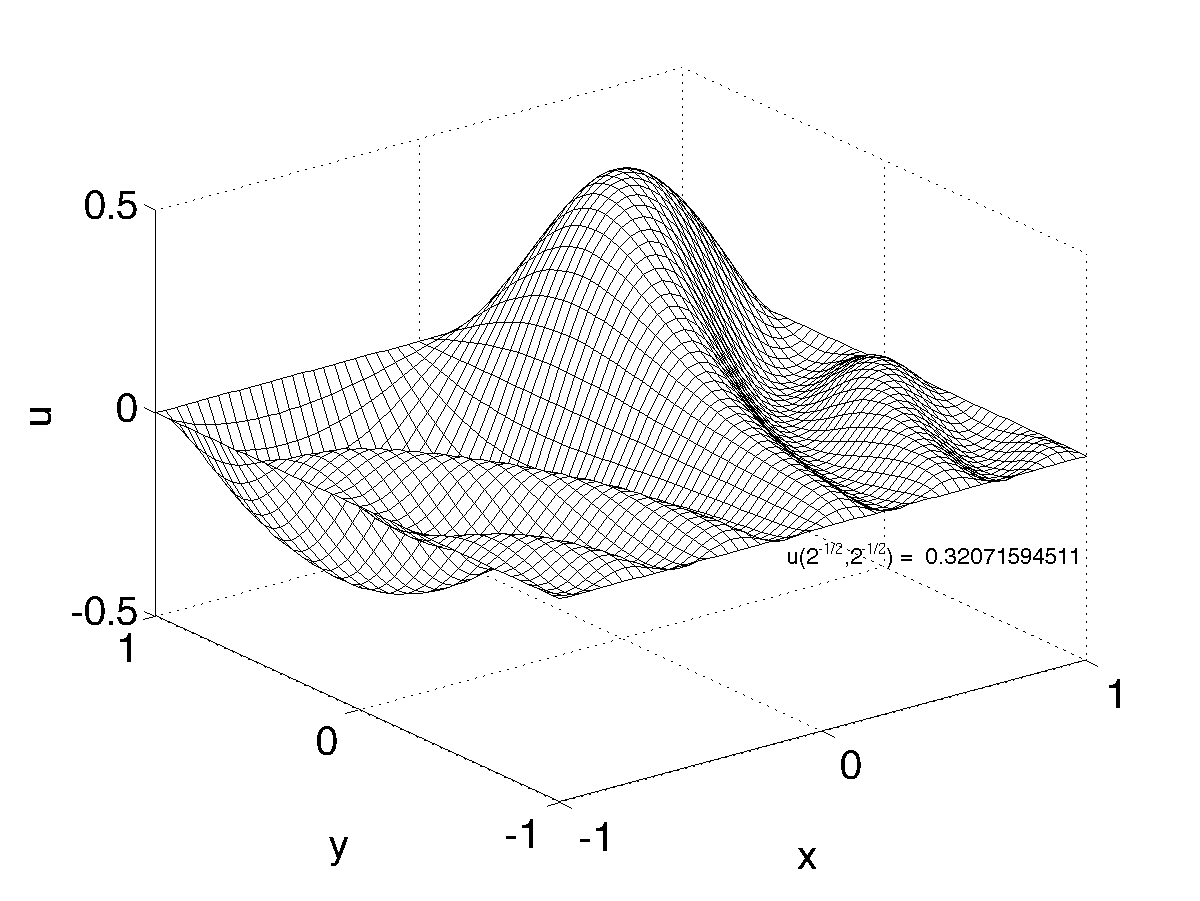
\includegraphics[width=\textwidth]{figures/SpectralElliptic}
      \end{center}
    \end{column}
  \end{columns}

\end{frame}

\begin{frame}
  \frametitle{Boundary conditions}

  \begin{center}
    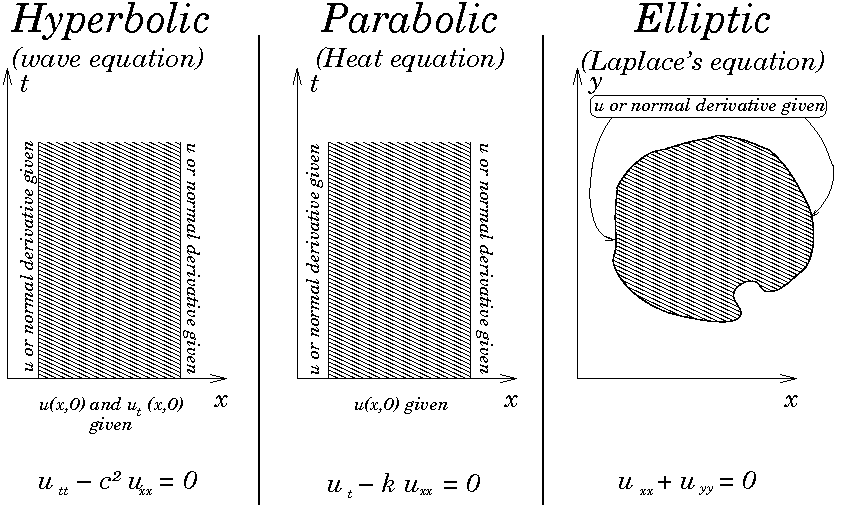
\includegraphics[width=0.9\textwidth]{figures/pde_summary}
  \end{center}

\end{frame}

\section{Elliptic equations}

\subsection{Finite difference methods for elliptic equations}

\begin{frame}
  \frametitle{Finite difference methods for elliptic equations}

  Take Poisson's equation with Dirichlet boundary conditions
  \begin{equation*}
    \left\{
      \begin{aligned}
        u_{x x} + u_{y y} & = f(x, y), && \text{in } \Omega, \\
        u\big |_{\partial\Omega} & = \phi(x, y), && \text{on }
        \partial\Omega
      \end{aligned}
    \right. .
  \end{equation*}
  Simple approach: replace all derivatives with finite difference
  equivalents. \pause

  \vspace{1ex}

  Directly generalizes BVPs. Algorithm:
  \begin{enumerate}
  \item<2-> Introduce grid covering $\Omega$.
  \item<3-> Convert PDE to linear system for unknown interior points.
  \item<4-> Solve the linear system.
  \end{enumerate} \pause[5]
  As in BVP case, boundary data is known through $\phi$.

\end{frame}

\begin{frame}
  \frametitle{The grid}

  \begin{columns}
    \begin{column}{0.5\textwidth}
      Assume that $\Omega$ is a rectangle:
      \begin{equation*}
        x \in [0,a], \quad y \in [0, b].
      \end{equation*}
      Use $n+2$ points in $x$, $m+2$ in $y$:
      \begin{align*}
        h_x & = \frac{a}{n + 1}, \\
        h_y & = \frac{b}{m + 1}.
      \end{align*}
      Location of $(i,j)$ grid point is
      \begin{equation*}
        \begin{pmatrix}
          x_{i} \\ y_{j}
        \end{pmatrix} =
        \begin{pmatrix}
          i h_x \\ j h_y
        \end{pmatrix}.
      \end{equation*}
    \end{column}
    \begin{column}{0.5\textwidth}
      \begin{center}
        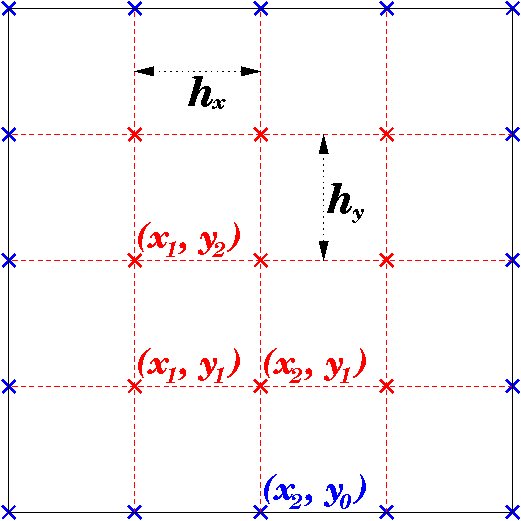
\includegraphics[width=\textwidth]{figures/Grid1_Elliptic}
      \end{center}
    \end{column}
  \end{columns}

\end{frame}

\begin{frame}
  \frametitle{Finite difference formula}

  Apply central differencing to PDE
  \begin{equation*}
    u_{x x} + u_{y y} = f
  \end{equation*}
  for the \emph{interior} points $0 < i < n+1$, $0 < j < m+1$. Result:
  \begin{align*}
    u_{x x} & = \frac{u_{i-1, j} + u_{i+1,j} - 2 u_{i,j}}{h_x^2} +
    {\cal O}(h_x^2), \\
    u_{y y} & = \frac{u_{i, j-1} + u_{i,j+1} - 2 u_{i,j}}{h_y^2} +
    {\cal O}(h_y^2).
  \end{align*} \pause

  Rearranging and defining $\alpha = ( h_x / h_y )^2$ gives
  \begin{equation*}
    \left[ u_{i-1, j} + u_{i+1,j} - 2 u_{i,j} \right] + \alpha \left[
      u_{i, j-1} + u_{i,j+1} - 2 u_{i,j} \right] = h_x^2 f_{i,j}
  \end{equation*}\pause

  System of $n \times m$ linear equations for $n \times m$ unknowns,
  as boundary data ($u_{0, j}$, $u_{n+1,j}$ etc.) is known.

\end{frame}

\begin{frame}
  \frametitle{Ordering}

  \begin{columns}
    \begin{column}{0.5\textwidth}
       Want to form a linear system
      \begin{equation*}
        A \bfm{u} = \bfm{F}.
      \end{equation*}
      But $u_{i,j}$ form a matrix, so re-order entries as vector of
      unknowns $\bfm{u}$. \pause

      \vspace{1ex}

      \emph{Natural ordering by columns}:
      \begin{equation*}
        u_k = u_{i, j}, \quad k \leftrightarrow j + m (i - 1).
      \end{equation*} \pause
      Natural ordering by \emph{rows}:
      \begin{equation*}
        u_k = u_{i, j}, \quad k \leftrightarrow i + n (j - 1).
      \end{equation*}
    \end{column}
    \begin{column}{0.5\textwidth}
      \begin{center}
        \includegraphics<1|handout:0>[width=\textwidth]{figures/Grid1_Elliptic}
        \includegraphics<2>[width=\textwidth]{figures/Grid3_Elliptic}
        \includegraphics<3|handout:0>[width=\textwidth]{figures/Grid4_Elliptic}
      \end{center}
    \end{column}
  \end{columns}

\end{frame}

\begin{frame}
  \frametitle{The matrix}

  Apply natural ordering by rows to equation
  \begin{equation*}
    \left[ u_{i-1, j} + u_{i+1,j} - 2 u_{i,j} \right] + \alpha \left[
      u_{i, j-1} + u_{i,j+1} - 2 u_{i,j} \right] = h_x^2 f_{i,j}.
  \end{equation*} \pause
  For $2 \times 3$ example in the notes have
  \begin{equation*}
    \bfm{u} = [u_{1,1} , u_{1,2} , u_{1,3} , u_{2,1} , u_{2,2} , u_{2,3}]^T
  \end{equation*}
  and the matrix $A$ given by
  {\small
    \begin{equation*}
      \begin{pmatrix}
        -2 ( 1 + \alpha ) & \alpha & 0 & 1 & 0 & 0 \\
        \alpha & -2 ( 1 + \alpha ) & \alpha & 0 & 1 & 0 \\
        0 & \alpha & -2 ( 1 + \alpha ) & 0 & 0 & 1 \\
        1 & 0 & 0 & -2 ( 1 + \alpha ) & \alpha & 0 \\
        0 & 1 & 0 & \alpha & -2 ( 1 + \alpha ) & \alpha \\
        0 & 0 & 1 & 0 & \alpha & -2 ( 1 + \alpha )
      \end{pmatrix}.
    \end{equation*}
  }
  The matrix is \emph{sparse} but not tridiagonal.

\end{frame}

\begin{frame}
  \frametitle{Boundary terms and the known vector}

  In constructing $A$, ignored known elements such as $u_{0,j}$, (will
  be moved to RHS). \pause  Construct $\bfm{F}$ for $2 \times 3$
  example with equation
  \begin{equation*}
    \left[ u_{i-1, j} + u_{i+1,j} - 2 u_{i,j} \right] + \alpha \left[
      u_{i, j-1} + u_{i,j+1} - 2 u_{i,j} \right] = h_x^2 f_{i,j}
  \end{equation*}
  and ordering
  \begin{equation*}
    \bfm{u} = [u_{1,1} , u_{1,2} , u_{1,3} , u_{2,1} , u_{2,2} , u_{2,3}]^T
  \end{equation*}
  to find
  \begin{equation*}
    \bfm{F} =
    \begin{pmatrix}
      h_x^2 f_{1,1} - u_{0,1} - \alpha u_{1,0} \\
      h_x^2 f_{1,2} - u_{0,2} \\
      h_x^2 f_{1,3} - u_{0,2} - \alpha u_{1,4} \\
      h_x^2 f_{2,1} - u_{3,1} - \alpha u_{2,0} \\
      h_x^2 f_{2,2} - u_{3,2} \\
      h_x^2 f_{2,3} - u_{3,3} - \alpha u_{2,4} \\
    \end{pmatrix}
  \end{equation*}

\end{frame}

\begin{frame}
  \frametitle{Example}

  \begin{columns}
    \begin{column}{0.4\textwidth}
      Solve
      %
      {\small
        \begin{equation*}
          u_{x x} + u_{y y} = -2 \pi^2 \sin(\pi x) \sin(\pi y)
        \end{equation*}%
      }
      %
      on $(x,y) \in [0,1]^2$ with trivial boundary conditions. \pause

      \vspace{1ex}

      Increasing resolution improves the accuracy \pause steadily
      \pause and we can see second order convergence.
    \end{column}
    \begin{column}{0.6\textwidth}
      \begin{center}
        \includegraphics<1|handout:0>[width=\textwidth]{figures/PoissonExact1}
        \includegraphics<2|handout:0>[width=\textwidth]{figures/PoissonExact2}
        \includegraphics<3|handout:0>[width=\textwidth]{figures/PoissonExact3}
        \includegraphics<4>[width=\textwidth]{figures/PoissonExactConvergence1}
      \end{center}
    \end{column}
  \end{columns}

\end{frame}

\begin{frame}
  \frametitle{Example: 2}

  \begin{columns}
    \begin{column}{0.4\textwidth}
      The equation
      %
      {\footnotesize
        \begin{align*}
          u_{x x} + u_{y y} & = x e^y, & (x,y) & \in [0,1]^2, \\
          u & = 0 & \text{on } x & = 0, \\
          u & = e^y & \text{on } x & = 1, \\
          u & = x & \text{on } y & = 0, \\
          u & = x e & \text{on } y & = 1,
        \end{align*}%
      }
      %
      is also straightforwardly solved. \pause

      \vspace{1ex}

      Increasing resolution improves the accuracy \pause steadily
      \pause and we can still see second order convergence.
    \end{column}
    \begin{column}{0.6\textwidth}
      \begin{center}
        \includegraphics<1|handout:0>[width=\textwidth]{figures/PoissonExactBound1}
        \includegraphics<2|handout:0>[width=\textwidth]{figures/PoissonExactBound2}
        \includegraphics<3|handout:0>[width=\textwidth]{figures/PoissonExactBound3}
        \includegraphics<4>[width=\textwidth]{figures/PoissonExactBoundExpConvergence1}
      \end{center}
    \end{column}
  \end{columns}

\end{frame}

\begin{frame}
  \frametitle{Iterative methods for the linear system}

  Have constructed a second order convergent method. But \emph{direct}
  matrix solver takes ${\cal O}(N^3)$ operations, so typically looking
  at ${\cal O}(n^6)$ operations! \pause Then consider extending to
  three dimensions... \pause

  \vspace{1ex}

  Instead note that the finite difference equations
  \begin{equation*}
    \left[ u_{i-1, j} + u_{i+1,j} - 2 u_{i,j} \right] + \alpha \left[
      u_{i, j-1} + u_{i,j+1} - 2 u_{i,j} \right] = h_x^2 f_{i,j}
  \end{equation*}
  in good form for an \emph{iterative} method. These often work well
  for sparse matrices, as here. \pause

  \vspace{1ex}

  Gauss-Seidel or variants on the SOR methods are frequently used for
  solving elliptic equations in this fashion.

\end{frame}

\begin{frame}
  \frametitle{Example}

  \begin{columns}
    \begin{column}{0.4\textwidth}
      The equation
      {\small
        \begin{equation*}
          u_{x x} + u_{y y} = -2 \pi^2 \sin(\pi x) \sin(\pi y)
        \end{equation*}}
      on $(x,y) \in [0,1]^2$ with trivial boundary conditions is
      straightforwardly solved. \pause

      \vspace{1ex}

      Increasing resolution improves the accuracy \pause steadily
      \pause and we can see second order convergence.
    \end{column}
    \begin{column}{0.6\textwidth}
      \begin{center}
        \includegraphics<1|handout:0>[width=\textwidth]{figures/PoissonGS1}
        \includegraphics<2|handout:0>[width=\textwidth]{figures/PoissonGS2}
        \includegraphics<3|handout:0>[width=\textwidth]{figures/PoissonGS3}
        \includegraphics<4>[width=\textwidth]{figures/PoissonGSConvergence1}
      \end{center}
    \end{column}
  \end{columns}

\end{frame}


\subsection{Spectral collocation methods}

\begin{frame}
  \frametitle{Collocation methods}

  \begin{columns}
    \begin{column}{0.35\textwidth}
      Collocation methods extend to elliptic equations. Work well on
      simple domains with smooth boundary conditions. \pause

      \vspace{1ex}

      Convergence is exceptionally fast; when these methods work,
      finite differences cannot compete.
%
%       For a good introduction see Trefethen's book, \emph{Spectral
%         Methods in Matlab}.
    \end{column}
    \begin{column}{0.65\textwidth}
      \begin{center}
        \includegraphics<1|handout:0>[width=\textwidth]{figures/SpectralElliptic}
        \includegraphics<2->[width=\textwidth]{figures/SpectralConvergenceElliptic}
      \end{center}
    \end{column}
  \end{columns}

\end{frame}

\section{Summary}

\subsection{Summary}

\begin{frame}
  \frametitle{Summary}

  \begin{itemize}
  \item Partial differential equations have (at least) two independent
    variables, either denoted $(x,y)$ for boundary value (elliptic)
    problems or $(t,x)$ for evolutionary (hyperbolic, parabolic)
    problems.
  \item Boundary conditions are required to specify a unique
    solution. In evolutionary problems the conditions at $t=0$ are
    called initial conditions.
  \item Elliptic equations are in some sense generalizations of
    boundary value problems.
  \item Introducing an evenly spaced grid and used central
    differencing leads to a set of finite difference equations.
  \item Using some natural ordering of the entries gives a linear
    system.
  \item The linear system is sparse and is best solved with iterative
    methods.
  \item Collocation methods, when they work, are much better.
  \end{itemize}

\end{frame}

\end{document}



%%% Local Variables:
%%% mode: latex
%%% TeX-master: t
%%% End:
